\documentclass[11pt]{article}
\usepackage[final]{acl}
\usepackage{times}
\usepackage{latexsym}
\usepackage[T1]{fontenc}
\usepackage[utf8]{inputenc}
\usepackage{microtype}
\usepackage{graphicx}
\usepackage{booktabs}
\usepackage{multirow}
\usepackage{tabularx}
\usepackage{enumitem}
\setlist{nosep, leftmargin=*}
\newcommand{\geov}{\textsc{Geo-v}}

\title{Order, Duration, or Melody? Probing What Phone Recognizers Use\\to Geolocate Haryanvi and Hindi-Belt Speech}

\author{Mohit Kumar Singh \qquad\qquad Nidhi Vaidya \\
  Speech Analysis and Linguistics (Monsoon 2026), IIIT Hyderabad \\
  Progress report, 3 November 2026}

\begin{document}
\maketitle

\begin{abstract}
PRiSM benchmarks phone recognizers and reports that, for locating where a Hindi-belt speaker is from, a probe
that reads the recognizer's predicted phones beats a probe that reads its hidden states. We test what the phone
string carries and whether the benchmark measures dialect at all. On PRiSM's own data we reproduce its transcript
probe (45.5 Recall@1 against the reported 45.7), but a voice embedding trained only to tell speakers apart
scores 55.1. On a
rebuilt copy of the task with known speakers, a lookup that knows only the speaker scores 98.0 and a lookup that
knows only which picture was described scores 61.8. Once test speakers are new, every probe on PRiSM's data falls
to the majority baseline. On our rebuild the transcript probes keep a small margin, mostly from the picture
described, and the gain that PRiSM's sequence model gets from phone order disappears. In the audio, Haryana
speakers hold voiceless stops 14\% longer than New Delhi speakers, but the recognizers rarely write this
lengthening. Representation probes are not yet run.
\end{abstract}

\section{Introduction}
PRiSM \citep{bharadwaj2026prism} benchmarks phone recognizers. One of its tasks, \geov{}, asks a probe to place
an utterance from the Hindi belt on the map, using the Vaani-Hi data \citep{ghosh2025vaani}. PRiSM probes each
recognizer in two ways. A transcript probe reads the predicted phone string; a representation probe reads the
recognizer's hidden states. The transcript probe has the lower mean error (146\,km against 253\,km), and the
authors suggest that phone order explains the gap.

The result is surprising, because only the representation probe hears the voice, the
intonation and the exact durations. We ask four questions. Does PRiSM's evaluation let probes recognise speakers or topics
in place of dialect (RQ0)? Does phone order carry location beyond which phones occur, on seen and on new speakers
(RQ1)? Do Haryana speakers lengthen consonants in the audio, and do the recognizers write the lengthening (RQ2)?
Do pitch and intensity contours add location information to the transcript probe (RQ3)?

This report covers the work up to the mid evaluation. The transcript, voice and prosody probes, the audit of
PRiSM's data and the acoustic study are complete. The representation probes are planned for November
(Section~\ref{sec:plan}).

\section{Related work}
\citet{foley2024where} geolocate speech from radio broadcasts and hold out whole stations, so that a model
cannot succeed by recognising a station. PRiSM's \geov{} split instead assigns utterances to train and test at
random within each pincode. A probe's score mixes what a representation encodes with what the probe can learn;
control tasks \citep{hewitt2019control} and description length \citep{voita2020mdl} separate the two. Speech
models encode phonetic detail differently in different layers \citep{pasad2021layerwise,wells2022phonetic}.
\citet{mishra2011dialects} compared seven Hindi dialects and found that they keep the
same basic sound inventory and differ in allophonic variation; for Haryanvi they report more open vowels and
retroflex /r/, /n/ and /l/. Dialects can also differ in how often phones occur and in their order
\citep{shim2024phonotactic}. PRiSM, citing \citet{devi2021haryanvi}, notes that speakers of the Bangru dialect of
Haryanvi double consonants that are single in standard Hindi, and Hindi geminates have longer closures than single consonants
\citep{ohala2007geminates}. Intonation also carries dialect identity
\citep{grabe2002intonational,vicenik2013intonation}.

\section{Data}
\label{sec:data}
Table~\ref{tab:data} compares the two versions of Vaani-Hi we use.

\paragraph{Our rebuild.} Access to PRiSM's copy came late, and that copy has no speaker labels, so most of our
analyses use a rebuild. We reran PRiSM's selection code on the public Vaani corpus at a fixed commit and
obtained 22,551 utterances (40.3 hours) from 26 pincodes in 9 states. A second machine produced the same files
bit for bit. Each Vaani file name contains a speaker code, and the rebuild has 1,570 speakers, with a median of 5 and at
most 257 utterances each.

\paragraph{PRiSM's release.} PRiSM's copy has 26,385 rows but only 21,481 distinct recordings. PRiSM's sampling
script writes the first 600 clips of each of a district's four shards to the same 600 file names, so the shards
overwrite each other's audio, but the metadata keeps one row per shard. In the release, 4,559 recordings appear in
two to four rows, often with different labels, and 28.0\% of test rows have their exact audio in training. The
largest class, pincode 171202 in Shimla, is placed in Afghanistan, 844\,km from its post offices, because PRiSM
averages the coordinates of the pincode's post offices and three of them have latitude and longitude swapped.

\paragraph{Splits.} PRiSM splits utterances at random within each pincode. Under this split, 97.9\% of test
utterances in our rebuild come from a speaker who is also in training. We add a speaker-disjoint split,
stratified by pincode, in which no test speaker appears in training. We call its test speakers new speakers.

\paragraph{Pictures.} Vaani speakers describe pictures, and 68\% of our utterances describe a picture of the
speaker's own district. The topic of an utterance can point to its location without any dialect
feature. The remaining utterances describe shared pictures that are not tied to a district.

\paragraph{Audio for duration.} Vaani-Hi has only 12 Haryana speakers. For RQ2 we use separate Vaani audio from
three Haryana districts (Rohtak, Jhajjar, Charkhi Dadri) and New Delhi, 23,963 utterances in all.

\begin{table}[t]
\centering\footnotesize
\begin{tabularx}{\linewidth}{@{}>{\raggedright\arraybackslash}Xrr@{}}
\toprule
 & Rebuild & Release \\
\midrule
Rows & 22,551 & 26,385 \\
Distinct recordings & 22,548 & 21,481 \\
Recordings in several rows & 3 & 4,559 \\
Hours of audio & 40.3 & -- \\
Speakers & 1,570 & not given \\
States / districts / pincodes & 9 / 18 / 26 & 10 / 20 / 30 \\
Test rows, PRiSM's split & 3,404 & 3,985 \\
Test speakers also in training, PRiSM's split & 97.9\% & all (est.) \\
Test speakers also in training, speaker-disjoint split & 0.0\% & -- \\
Test clips whose exact audio is in training & 0 & 28.0\% \\
\bottomrule
\end{tabularx}

\caption{The two versions of Vaani-Hi. PRiSM's release has no speaker labels; its speaker overlap is estimated
from voice embeddings calibrated on our rebuild.}
\label{tab:data}
\end{table}

\begin{figure*}[t]
\centering
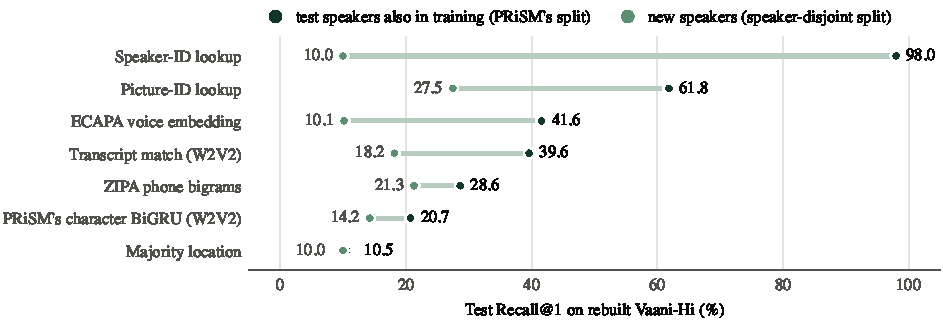
\includegraphics[width=\textwidth]{../results/figures/fig_lookups.pdf}
\caption{Under both splits the best lookup scores above every trained probe, though no lookup uses any
information about dialect. All scores fall when test speakers are new, and the voice embedding falls to the majority baseline. Trained
probes show the mean over seeds.}
\label{fig:lookups}
\end{figure*}

\section{Method}
\label{sec:method}
\paragraph{Probes.} Every probe predicts a point on the globe and is trained with PRiSM's angular loss. The
transcript probes read the phone strings of two recognizers, W2V2 and ZIPA \citep{zhu2025zipa}, produced with
PRiSM's own code. They are PRiSM's two-layer BiGRU over characters, the same BiGRU over phones, the same BiGRU
over phones shuffled within each utterance, and small MLPs over the relative frequencies of phones or characters (unigrams)
or of adjacent pairs (bigrams). Shuffling keeps which phones occur and removes their order, so the BiGRU against the
shuffled BiGRU measures what order adds. A voice probe is an MLP over ECAPA-TDNN embeddings
\citep{desplanques2020ecapa}, which are trained to tell speakers apart and so capture the voice and the recording
channel. A prosody probe is a BiGRU
over F0, voicing and intensity contours from Praat \citep{jadoul2018parselmouth,boersma2024praat}, also fused
with the transcript BiGRU by averaging their predictions with a weight chosen on validation data.

\paragraph{References.} Four references learn nothing about dialect. The majority baseline always predicts the
most common training location. A speaker-ID lookup predicts the most common training location of the test
utterance's speaker, and a picture-ID lookup does the same for the picture. A transcript matcher finds the most
similar training transcript (character n-grams) and copies its location.

\paragraph{Metrics and statistics.} Recall@1, PRiSM's metric, is the share of test utterances for which, of all
distinct test locations, the one nearest to the prediction is the true one. We also report mean error in km.
Each probe is trained with five seeds; the BiGRUs have two or three so far and the prosody BiGRU one. Comparisons between probes are paired on the
same test utterances, with 95\% confidence intervals from a bootstrap over speakers, because utterances of one
speaker are not independent. We also measure how many bits a probe saves when coding the pincode
(minimum description length, \citealp{voita2020mdl}).

\paragraph{Duration.} Forced alignment of the standard spelling \citep{pratap2024mms} locates single voiceless
stops between vowels. Praat's voicing and burst landmarks give each stop's voiceless interval and closure. A
mixed model compares Haryana with New Delhi, with a fixed effect per word, a control for speaking rate and a
random intercept per speaker. Lexical geminates (e.g., \textit{acch\=a}) check that the measure tracks length.

\begin{table*}[t]
\centering\small
\begin{tabular}{lrrrr}
\toprule
 & \multicolumn{2}{c}{PRiSM's split} & \multicolumn{2}{c}{New speakers} \\
\cmidrule(lr){2-3}\cmidrule(lr){4-5}
Probe & R@1 & km & R@1 & km \\
\midrule
\multicolumn{5}{l}{\textit{References that learn nothing about dialect}} \\
\quad Majority location & 10.5 & 660 & 10.0 & 675 \\
\quad Speaker-ID lookup & 98.0 & 12 & 10.0 & 675 \\
\quad Picture-ID lookup & 61.8 & -- & 27.5 & -- \\
\quad Transcript match (W2V2) & 39.6 & 452 & 18.2 & 590 \\
\midrule
\multicolumn{5}{l}{\textit{Voice and prosody}} \\
\quad ECAPA voice embedding & $41.6 \pm 1.6$ & 169 & $10.1 \pm 0.6$ & 435 \\
\quad Pooled prosody statistics & $5.5 \pm 0.7$ & 571 & $4.8 \pm 0.4$ & 595 \\
\midrule
\multicolumn{5}{l}{\textit{Transcript probes, W2V2}} \\
\quad phone unigram & $15.5 \pm 1.1$ & 440 & $12.6 \pm 0.7$ & 469 \\
\quad phone bigram & $27.9 \pm 0.8$ & 360 & $17.8 \pm 1.7$ & 436 \\
\quad character BiGRU (PRiSM's) & $20.7 \pm 1.2$ & 374 & $14.2 \pm 0.5$ & 434 \\
\quad phone BiGRU & $21.4 \pm 1.3$ & 384 & $11.8 \pm 1.3$ & 445 \\
\quad shuffled phone BiGRU & $18.3 \pm 0.0$ & 437 & $15.7 \pm 0.5$ & 468 \\
\midrule
\multicolumn{5}{l}{\textit{Transcript probes, ZIPA}} \\
\quad phone unigram & $15.2 \pm 0.5$ & 443 & $12.7 \pm 1.0$ & 472 \\
\quad phone bigram & $28.6 \pm 0.8$ & 344 & $21.3 \pm 1.0$ & 403 \\
\quad character BiGRU (PRiSM's) & $21.2 \pm 0.2$ & 362 & $13.9 \pm 1.4$ & 423 \\
\quad phone BiGRU & $21.9 \pm 0.5$ & 366 & $16.0 \pm 2.1$ & 425 \\
\quad shuffled phone BiGRU & $18.6 \pm 0.3$ & 441 & $15.6 \pm 2.5$ & 468 \\
\bottomrule
\end{tabular}

\caption{Test Recall@1 (mean $\pm$ sd over seeds) and mean error in km of the seed ensemble on our rebuild.
BiGRUs have two seeds so far. The picture-ID lookup has no km value because it predicts a pincode, not a point.}
\label{tab:main}
\end{table*}

\section{Results}
\label{sec:results}
Table~\ref{tab:main} gives every probe on our rebuild under both splits, and Figure~\ref{fig:lookups} shows the
main comparison.



\subsection{RQ0: speakers and topic}
Under PRiSM's split, a lookup that knows only the speaker reaches 98.0 Recall@1, against 10.5 for the majority
baseline. The ECAPA voice embedding reaches 41.6. When every speaker is relabelled with another speaker's
location, a control task that keeps speaker identity and removes dialect, ECAPA still scores 33.2 against a
control majority of 14.0. Most of its score is speaker recognition. On new speakers ECAPA scores 10.1, the
majority level.

The transcripts identify speakers too. The transcript matcher reaches 39.6 under PRiSM's split, and for 25\% of
test utterances its nearest training transcript comes from the same speaker; by chance this would happen for
0.3\%. On new speakers it scores 18.2.

A lookup by picture ID scores 61.8 [58.9, 64.7] under PRiSM's split, above
PRiSM's reported 45.7, and 27.5 [20.7, 36.5] on new speakers, above every transcript probe. Each
district-specific picture is described only by speakers of that district, so naming the picture names the place. For new speakers on shared pictures, the same
lookup scores 10.1, below that subset's majority of 21.3, so these pictures give no location. When transcript
probes are trained and tested on shared pictures only, none beats the majority on Recall@1 for new speakers.
With shared speakers, phone bigrams still beat it by 13.7 [8.2, 19.1] points for W2V2 and 12.5 [7.6, 17.5] for ZIPA.

On new speakers the best transcript probe is ZIPA phone bigrams, at 21.3 Recall@1, 10.6 [6.2, 15.9] points above
the majority baseline. Since no transcript probe beats the majority on shared pictures from new speakers, most of this margin comes
from what speakers describe.

\begin{table*}[t]
\centering\small
\begin{minipage}{0.8\textwidth}
\begin{tabularx}{\linewidth}{@{}>{\raggedright\arraybackslash}Xrrr@{}}
\toprule
Probe & Released & Corrected & New speakers \\
\midrule
Majority location & 7.6 & 7.5 & 6.8 \\
Transcript match & 58.9 & 57.5 & 9.6 \\
ECAPA voice & $55.1 \pm 1.4$ & $54.0 \pm 2.0$ & $3.4 \pm 0.5$ \\
W2V2 phone bigram & $59.6 \pm 0.7$ & $57.3 \pm 1.6$ & $8.7 \pm 0.6$ \\
ZIPA phone bigram & $59.5 \pm 1.0$ & $59.8 \pm 0.6$ & $9.2 \pm 1.3$ \\
PRiSM's char.\ BiGRU & $45.5 \pm 1.1$ & $47.0 \pm 0.7$ & $8.0 \pm 0.4$ \\
Phone BiGRU & -- & $46.6 \pm 0.8$ & $9.0 \pm 0.8$ \\
Shuffled phone BiGRU & -- & $29.6 \pm 1.3$ & $8.0 \pm 1.0$ \\
ZIPA char.\ BiGRU & -- & -- & -- \\
ZIPA phone BiGRU & -- & -- & -- \\
ZIPA shuffled phone BiGRU & -- & -- & -- \\
\bottomrule
\end{tabularx}

\caption{Test Recall@1 on PRiSM's release (mean $\pm$ sd over seeds). The first column uses the data and split as
released, the second the corrected rows under PRiSM's split, and the third the corrected rows with new speakers,
found by clustering voices. The corrected rows keep one row per recording, drop conflicting labels and put Shimla
at its post offices.}
\label{tab:release}
\end{minipage}
\end{table*}

\subsection{PRiSM's release}
With PRiSM's settings and our code, PRiSM's character BiGRU scores 45.5\,$\pm$\,1.1 Recall@1 on its own data and
split, against the 45.7 it reports (Table~\ref{tab:release}). The ECAPA voice
embedding reaches 55.1 and the transcript matcher 58.9, though neither can know dialect.

We built a corrected version with one row per recording, dropping recordings whose copies carry different
pincodes and moving Shimla to its post offices (19,731 rows). The release has no speaker labels, so we clustered
the ECAPA embeddings into 375 pseudo-speakers. The same clustering, applied to our rebuild where speakers are
known, leaves 2.1\% of test speakers in training. On the corrected rows the scores stay close to the released
ones under PRiSM's split. Under the speaker-disjoint split every probe falls to between 3.4 and 9.6 Recall@1,
around the majority of 6.8. Removing duplicate audio changes little; removing shared speakers removes almost
everything.


\subsection{RQ1: phone order}
Figure~\ref{fig:order} shows what phone order adds, paired on the same test utterances. On the corrected release,
PRiSM's BiGRU over phones beats the same BiGRU on shuffled phones by 18.6 [15.5, 22.3] points when speakers are
shared, and by $-$0.3 [$-$3.5, 2.4] on new speakers. On our rebuild the gain is smaller with shared speakers
(3.9 for W2V2, 4.3 for ZIPA) and absent on new speakers ($-$3.5 [$-$6.5, $-$1.0] and 0.4 [$-$1.9, 2.9]).

On our rebuild, phone bigrams beat phone unigrams on new speakers by 4.8
[2.6, 6.9] points for W2V2 and 7.8 for ZIPA, and phones beat characters by 3.5 [2.1, 5.1] for W2V2. On the
release with new speakers the bigram gain is 1.8 [$-$0.9, 4.7], from only 59 test pseudo-speakers. Description
length agrees with the rebuild result: ZIPA phone bigrams save 7.9\,kbits over the location prior on new speakers,
against 21.0\,kbits under PRiSM's split.

\begin{figure}[t]
\centering
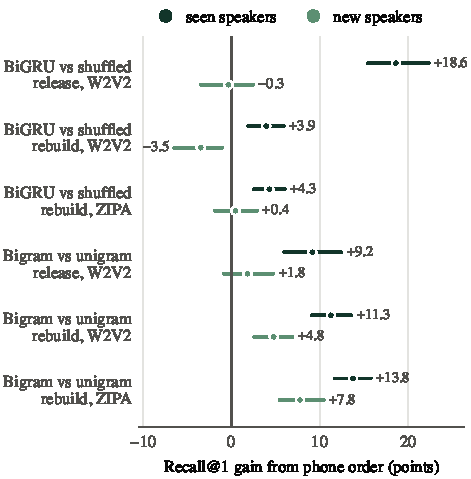
\includegraphics[width=\columnwidth]{../results/figures/fig_order.pdf}
\caption{Recall@1 gain from phone order, with 95\% confidence intervals. The BiGRU gains from order only when test
speakers were seen in training.}
\label{fig:order}
\end{figure}

\subsection{RQ2: consonant duration}
We measured 26,033 single voiceless stops between vowels, from 3,003 speakers. In Haryana their voiceless
interval is $\times$1.14 [1.11, 1.18] as long as in New Delhi, and their closure $\times$1.26 [1.21, 1.31]
(Table~\ref{tab:gem}). The effect appears in each Haryana district on its own ($\times$1.13 to $\times$1.15),
in 45 of 57 words, and in speaker means without any model ($\times$1.14). Lexical geminates are $\times$1.59
[1.51, 1.67] as long as single stops, so the measure tracks length, and Haryana's single stops move about a quarter of
the way to geminate length.

W2V2 writes a doubled consonant for only 1.0\% of the Haryana stops and
ZIPA for 1.9\%. W2V2's doubled stops are the longer ones (AUC 0.73 for predicting doubling from the voiceless
interval); ZIPA's are not (0.46). Across all consonants, W2V2 doubles fewer in Haryana than in other states
(1.00\% against 1.17\%, $p = 0.012$), and ZIPA shows no difference (1.63\% against 1.82\%, $p = 0.30$). A heuristic syllabification of the
recognizer strings, a syllable-level view of doubling, gives Haryana a share of closed
syllables inside the range of the other states (17.1\% against 16.4--20.0\% for W2V2, 20.0\% against
18.2--22.4\% for ZIPA). Whether the probes use the lengthening is not yet tested.

\begin{table*}[t]
\centering\small
\begin{tabular}{lrrr}
\toprule
Model & Haryana / New Delhi & 95\% CI & tokens \\
\midrule
voiceless interval (primary) & $\times$1.142 & [1.106, 1.178] & 26,033 \\
voiceless interval, no rate control & $\times$1.133 & [1.098, 1.169] & 26,033 \\
voiceless interval, all contexts (sensitivity: includes stops after a deleted schwa) & $\times$1.141 & [1.108, 1.175] & 33,333 \\
closure, tokens with a burst & $\times$1.256 & [1.208, 1.307] & 26,033 \\
closure, clear bursts only (rise >= 6 dB, drop >= 10 dB) & $\times$1.269 & [1.215, 1.324] & 9,340 \\
\midrule
lexical geminate / single (New Delhi) & $\times$1.59 & [1.51, 1.67] & \\
\bottomrule
\end{tabular}

\caption{Haryana against New Delhi, as multiplicative effects from mixed models with 95\% confidence intervals.
The last row is the validity check on lexical geminates.}
\label{tab:gem}
\end{table*}

\subsection{RQ3: intonation}
Pooled prosody statistics score below the majority under both splits (4.8 Recall@1 on new speakers). A BiGRU over
the contours, with one seed so far, scores 11.3 on new speakers against a majority of 10.0, a difference of 1.3
[$-$5.1, 7.8]. Fused with the ZIPA phone BiGRU, it lowers the mean error from 441 to 426\,km ($-$14.9 [$-$21.6,
$-$8.1]) and leaves Recall@1 unchanged within its interval ($-$1.2 [$-$3.4, 0.8]).

\subsection{Checks of our own split}
Speaker codes come from file names, so one person or one phone can appear under several codes. We grouped codes of
one district whose voice embeddings are as close as two halves of one speaker's recordings. This merges 1,570
codes into 1,327 groups. In our speaker-disjoint split, 49 of 223 test speakers have such a look-alike code in
training. ECAPA's small gain over the majority on new speakers comes from them: $+$9.1 on their utterances and
$-$4.2 [$-$12.1, 2.2] on the rest. The transcript probes keep their gain on the rest (ZIPA phone bigrams $+$11.6
[5.2, 17.6]). The prosody BiGRU's distance gain also shrinks without look-alike speakers, from 132 to 48\,km
[$-$14, 123]. The fusion gain stays at $-$12.9\,km [$-$20.0, $-$5.1] without them.

Against the densest cluster of each pincode's post offices, PRiSM's recipe places two of our pincodes far off,
454552 (Dhar) by 266\,km and 834008 (Ranchi) by 61\,km. Recall@1 compares the prediction with the nearest
candidate location, so it changes little; the km errors include the offset.

\section{Discussion}
\label{sec:discussion}
On PRiSM's own data a voice embedding beats the transcript probe that PRiSM reports, and once speakers are new,
every probe falls close to the majority. PRiSM's comparison of the two probes rests on a split that rewards
recognising speakers. The gain from phone order that PRiSM points to appears only when test speakers were seen in
training. A probe that memorises each speaker's phone sequences would produce this pattern.

On new speakers, transcripts keep a small advantage over the majority, and most of it is the picture being
described. Bigram bags keep some gain on new speakers in our rebuild, but bigrams also identify words, and on
shared pictures from new speakers no transcript probe beats the majority. We cannot yet say how much of the bigram gain is dialect.

Haryana speakers lengthen voiceless stops,
the recognizers rarely write the lengthening, and so a transcript probe cannot use it. Whether the recognizers'
hidden states keep it, and whether a representation probe would then do better than a transcript probe on new
speakers, is the main open question.

\section{Status and plan}
\label{sec:plan}
So far we have rebuilt the dataset and its speaker-disjoint split, transcribed 72,899 utterances with two
recognizers, trained 392 probe runs, audited and corrected PRiSM's release, and measured 26,033 stops. The prosody
BiGRU and its fusion ran on the Ada cluster.

The representation probes have not run, because their cached hidden states did not fit the storage quota
available to us on Ada. The BiGRUs need three more seeds and the prosody BiGRU four more. Both authors still have
to check 50 measured stops by hand, without seeing the automatic measurements.

For the final evaluation on 4 December we plan to run PRiSM's representation probe on the last layer of three
recognizers, then order-aware representation probes across layers. All probes will then be rerun on a stricter
benchmark that we have already built and tested. It uses five-fold cross-validation over speaker groups, so that
every speaker is tested once, and corrected coordinates, and it has a second track restricted to shared pictures.

\section*{Limitations}
Vaani-Hi has only 12 Haryana speakers, and New Delhi stands for standard Hindi only approximately. On PRiSM's
release the speakers are estimated from voice embeddings, not known. The BiGRU results use two or three seeds and
the prosody BiGRU one. The acoustic landmarks are automatic and not yet checked by hand, and recognizer output is
not a phonetic gold standard.

\section*{Ethics}
Vaani is released under CC-BY 4.0 with speaker consent. We report only aggregate results and make no attempt to
identify speakers.

\bibliography{custom}
\end{document}
